% ==================================================================================
% W-DsgDetr Method — Detailed Technical Report
% Target Venue: NeurIPS
% ==================================================================================
\documentclass{article}

% Uncomment if neurips_2026.sty is available
% \usepackage[preprint]{neurips_2026}
% Fallback to standard margins if neurips is unavailable:
\usepackage[margin=1in]{geometry}

\usepackage[utf8]{inputenc}
\usepackage{amsmath,amssymb,amsfonts}
\usepackage{graphicx}
\usepackage{booktabs}
\usepackage{algorithm}
\usepackage{algpseudocode}
\usepackage{bm}
\usepackage{xcolor}
\usepackage{tikz}
\usetikzlibrary{arrows.meta,positioning,shapes.geometric,fit,calc,backgrounds}

\newcommand{\mR}{\mathbb{R}}
\newcommand{\op}[1]{\operatorname{#1}}
\newcommand{\mat}[1]{\bm{#1}}

\title{W-DsgDetr: World Scene Graph Generation with Explicit Temporal Tracking}
\author{Anonymous Authors}

\begin{document}

\maketitle

% ====================================================================================
\section{Introduction}
\label{sec:intro}
% ====================================================================================

The W-DsgDetr method is a world-aware adaptation of the DSG-DETR video scene graph model. The primary distinction between the W-STTran family and the W-DsgDetr family is the inclusion of explicit temporal object tracking. While W-STTran models rely strictly on a zero-order hold memory buffer and spatial graph networks, W-DsgDetr incorporates a \emph{TemporalObjectEncoder} that refines per-object representations across time using temporal self-attention.

This architecture isolates the benefit of temporal object tracking for WorldSGG. Like the base W-STTran, it does not utilize explicit camera pose or object motion encoders, ensuring that any performance gains are attributable directly to the TemporalObjectEncoder and the cross-frame TemporalEdgeAttention. W-DsgDetr employs a FasterRCNN-ResNet50 backbone.

% ====================================================================================
\section{Pipeline Overview}
\label{sec:pipeline}
% ====================================================================================

The dataflow of W-DsgDetr is depicted in Figure~\ref{fig:pipeline_wdsgdetr}. After extracting structural geometry and buffering visual features, tokens are processed across the temporal dimension for each object independently, followed by spatial reasoning and temporal edge-level attention.

\begin{figure}[h]
\centering
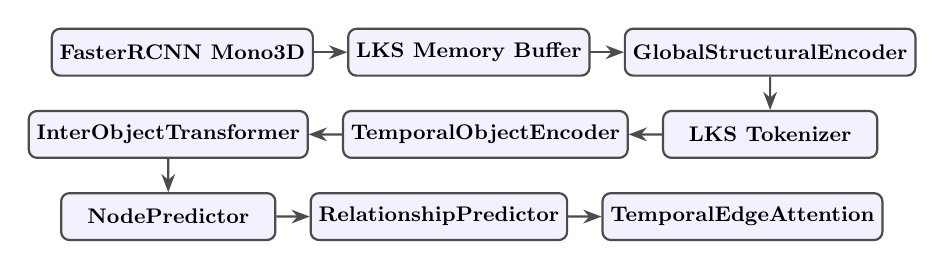
\begin{tikzpicture}[
  scale=0.85, transform shape, >=Stealth,
  block/.style={draw=black!70, rounded corners=3pt, line width=0.8pt, fill=blue!5, minimum width=3.2cm, minimum height=0.7cm, font=\small\bfseries, align=center},
  arrow/.style={->, thick, black!70}
]

\node[block] (mono) {FasterRCNN Mono3D};
\node[block, right=0.5cm of mono] (buffer) {LKS Memory Buffer};
\node[block, right=0.5cm of buffer] (gse) {GlobalStructuralEncoder};
\node[block, below=0.5cm of gse] (tok) {LKS Tokenizer};
\node[block, left=0.5cm of tok] (toe) {TemporalObjectEncoder};
\node[block, left=0.5cm of toe] (iot) {InterObjectTransformer};
\node[block, below=0.5cm of iot] (np) {NodePredictor};
\node[block, right=0.5cm of np] (rp) {RelationshipPredictor};
\node[block, right=0.5cm of rp] (tea) {TemporalEdgeAttention};

\draw[arrow] (mono) -- (buffer);
\draw[arrow] (buffer) -- (gse);
\draw[arrow] (gse) -- (tok);
\draw[arrow] (tok) -- (toe);
\draw[arrow] (toe) -- (iot);
\draw[arrow] (iot) -- (np);
\draw[arrow] (np) -- (rp);
\draw[arrow] (rp) -- (tea);

\end{tikzpicture}
\caption{The W-DsgDetr pipeline. It introduces explicit per-object tracking via the TemporalObjectEncoder prior to global spatial reasoning.}
\label{fig:pipeline_wdsgdetr}
\end{figure}

% ====================================================================================
\section{LKS Memory Buffer}
\label{sec:lks}
% ====================================================================================

To maintain object representations during occlusion or egress from the camera view, W-DsgDetr uses a zero-order hold buffer. The buffered feature for object $n$ at frame $t$ is:
\begin{equation}
    \mat{m}_n^{(t)} = \begin{cases}
        \mat{f}_n^{(t)} & \text{if visible at } t, \\
        \mat{f}_n^{(\tau^*)} & \text{where } \tau^* = \arg\min_{\tau:\text{vis}(n,\tau)} |t - \tau|, \\
        \bm{0} & \text{if never seen}.
    \end{cases}
    \label{eq:lks_buffer}
\end{equation}
The temporal staleness $\Delta_n^{(t)} = |t - \tau^*|$ acts as a learned confidence signal.

% ====================================================================================
\section{GlobalStructuralEncoder and Tokenizer}
\label{sec:gse_tok}
% ====================================================================================

The \emph{GlobalStructuralEncoder} generates structural tokens from 3D object bounding boxes. The 8 box corners $\mat{c}_{n,i}$ are zero-centered, flattened, concatenated with the absolute center $\bar{\mat{c}}_n$, and passed through an MLP:
\begin{equation}
    \mat{g}_n = \op{MLP}_{\text{obj}}\bigl([\op{flatten}(\tilde{\mat{c}}_{n,i}) \;\|\; \bar{\mat{c}}_n]\bigr) \in \mR^{d_{\text{struct}}}.
    \label{eq:gse_obj}
\end{equation}
The Tokenizer then fuses geometry, the LKS buffer, and staleness:
\begin{equation}
    \mat{x}_n^{(t)} = \op{FusionProj}\bigl([\mat{g}_n^{(t)} \;\|\; \mat{m}_n^{(t)} \;\|\; \log(\Delta_n^{(t)} + 1)]\bigr) \in \mR^{d_{\text{model}}}.
    \label{eq:tokenizer}
\end{equation}

% ====================================================================================
\section{TemporalObjectEncoder}
\label{sec:toe}
% ====================================================================================

The distinguishing component of W-DsgDetr is the \emph{TemporalObjectEncoder}. For each object $n$, it collects the $T$-length sequence of representations across the video and processes them using a standard Transformer encoder.

We add sinusoidal temporal positional encodings $\mat{PE}_{\text{sin}}(t)$ to sequence elements:
\begin{equation}
    \hat{\mat{X}}_n = \op{TransformerEncoder}\bigl(\{\mat{x}_n^{(t)} + \mat{PE}_{\text{sin}}(t)\}_{t=1}^T,\; \text{mask}=\text{pad\_mask}_n\bigr),
    \label{eq:toe}
\end{equation}
where the padding mask excludes entirely invalid frames for that object. The resulting sequence replaces the original input features. This enables the model to interpolate and contextualize representations across time.

% ====================================================================================
\section{InterObjectTransformer and Predictors}
\label{sec:iot_predictors}
% ====================================================================================

The temporally-refined tokens $\hat{\mat{X}}^{(t)}$ are passed through the \emph{InterObjectTransformer} for intra-frame spatial reasoning. Additive pairwise spatial positional embeddings $\mat{S}^{(t)}$ provide 3D relational biases:
\begin{equation}
    \mat{H}^{(t)} = \op{TransformerEncoder}\bigl(\hat{\mat{X}}^{(t)} + \mat{S}^{(t)},\; \text{mask}=\overline{\mat{v}}^{(t)}\bigr).
    \label{eq:iot}
\end{equation}

The \emph{Node Predictor} outputs class logits $\hat{\mat{Y}}^{\text{obj}}$. Next, the \emph{Relationship Predictor} forms initial relationship tokens $\mat{r}_{po}$ from node features and union boxes, refines them via relationship self-attention, and produces edge predictions.

Finally, the \emph{TemporalEdgeAttention} module aggregates these relationship tokens $\mat{r}_{po}$ for unique object pairs across time. Using a temporal positional embedding $\mat{e}_\tau$, it performs cross-frame edge attention to enforce temporal consistency:
\begin{equation}
    \tilde{\mat{r}}_{po}^{(t)} = \op{TemporalEncoder}\bigl(\{{\mat{r}}_{po}^{(\tau)} + \mat{e}_{\tau}\}_{\tau \in \mathcal{T}_{po}}\bigr).
    \label{eq:tea}
\end{equation}

% ====================================================================================
\section{Loss Function}
\label{sec:loss}
% ====================================================================================

The loss incorporates visible (clean GT) and unseen (VLM pseudo-labeled) pairs:
\begin{equation}
    \mathcal{L}_{\text{W-DsgDetr}} = \sum_{r \in \{\text{att, spa, con}\}} \bigl(\mathcal{L}_{r}^{\text{vis}} + \mathcal{L}_{r}^{\text{unseen}}\bigr) + \mathcal{L}_{\text{node}}.
    \label{eq:loss}
\end{equation}
Unseen pair losses are weighted by $\lambda_{\text{vlm}}$ and utilize label smoothing.

% ====================================================================================
\section{Algorithm: Forward Pass}
\label{sec:algorithm}
% ====================================================================================

\begin{algorithm}[h]
\caption{W-DsgDetr Forward Pass}
\begin{algorithmic}[1]
\Require $\mat{f}_{\text{all}}$ (visual), $\mat{C}_{\text{all}}$ (OBBs)
\Ensure $\hat{\mat{y}}_{\text{att}}, \hat{\mat{y}}_{\text{spa}}, \hat{\mat{y}}_{\text{con}}$
\State $(\mat{m}_{\text{all}}, \bm{\Delta}_{\text{all}}) \gets \text{LKS\_Buffer}(\mat{f}_{\text{all}})$
\State $\mat{G}_{\text{all}} \gets \text{GlobalStructuralEncoder}(\mat{C}_{\text{all}})$
\State $\mat{X} \gets \text{Tokenizer}(\mat{G}_{\text{all}}, \mat{m}_{\text{all}}, \log \bm{\Delta}_{\text{all}})$
\State $\hat{\mat{X}} \gets \text{TemporalObjectEncoder}(\mat{X})$ \Comment{Explicit temporal tracking}
\State $\mat{H} \gets \text{InterObjectTransformer}(\hat{\mat{X}})$
\State $\hat{\mat{Y}}^{\text{obj}} \gets \text{NodePredictor}(\mat{H})$
\State $\mat{R} \gets \text{RelationshipFormationAndSelfAttention}(\mat{H}, \hat{\mat{Y}}^{\text{obj}})$
\State $\tilde{\mat{R}} \gets \text{TemporalEdgeAttention}(\mat{R})$
\State $(\hat{\mat{y}}_{\text{att}}, \hat{\mat{y}}_{\text{spa}}, \hat{\mat{y}}_{\text{con}}) \gets \text{PredictionHeads}(\tilde{\mat{R}})$
\State \Return $\hat{\mat{y}}_{\text{att}}, \hat{\mat{y}}_{\text{spa}}, \hat{\mat{y}}_{\text{con}}$
\end{algorithmic}
\end{algorithm}

\end{document}
